\documentclass[11pt]{article}
\usepackage{balance,graphics,times,setspace}
\usepackage{hyperref,graphicx,sidecap}
\usepackage[margin=1in]{geometry}
\usepackage[inline]{enumitem}
\usepackage[tiny,compact]{titlesec}

\setlength{\parskip}{.4em}

\newlist{inlinelist}{enumerate*}{1}
\setlist*[inlinelist,1]{
  label=\arabic*),
}

\setlist[itemize]{itemsep=0pt,topsep=0pt,parsep=0pt}
\setenumerate{itemsep=0pt,topsep=0pt,parsep=0pt}
\newcommand{\sectitle}[1]{\textit{#1}}

\begin{document}

\section*{Collective Action and Governance in an Online Piecework Economy}

\begin{itemize}[leftmargin=0em,label={}]
  \item Michael Bernstein, Computer Science, Stanford University
  \item Margaret Levi, Political Science and CASBS, Stanford University
\end{itemize}

\section*{Abstract:} 
The digital gig economy has led to a resurgence of piecework.
Without shared factories and water coolers,
how do digital pieceworkers coordinate,
build solidarity,
and take collective action?
We will engage in fieldwork with digital pieceworkers who work in data entry,
domestic services,
and on--demand driving to understand how they counter algorithmic systems and engage in collective behavior.
We will then design and launch a new collectively--governed platform for domestic workers,
in collaboration with Fair Care Labs at the NDWA
(National Domestic Workers Alliance).
Our goal is to both understand the factors that drive collective behavior in supposedly--distributed gig platforms,
and to introduce new designs and infrastructure that enable the growth of worker collective action in the digital piecework
(gig)
economy.
Our results shed light on the strengths and weaknesses of  digital piecework cooperativism,
as well as the policies necessary for it to succeed.

\section*{Relationship to previously funded work:}
PIs Bernstein,
Levi,
Johari and Valentine have an ongoing funded Cyber project titled ``Cyber Work: The Future of Networked Labor".
This project outlined major goals:
\begin{inlinelist}
\item ethnographic studies of online work practice,
\item the creation of crowd organizations,
\item collective action,
and
\item new labor platforms
\end{inlinelist}.
The project was scoped too ambitiously for the funding available last year,
requesting \$1.2 million over three years.
Thus, we have split out part of
(1) and all of
(3) into this separate proposal.
(2) and (4) are making rapid progress under the existing funding,
and currently have significant publications in preparation and under review,
as well as an alpha version of the platform launched.
If the committee wishes to fund this proposal,
we are comfortable with either pitching it as a separate proposal or folding it into the existing Cyber Work proposal as part of a renewal request.
The timing of the funding start date is flexible.

\begin{itemize}[leftmargin=0em,label={}]
\item Proposed budget: \$100,000 per year
\item Collaborators: Ali Alkhatib, Niloufar Salehi
\end{itemize}
\thispagestyle{empty}
\pagebreak
\clearpage
\setcounter{page}{1}

Piecework has historically disempowered workers and empowered employers.
Subdividing work and paying per task drives employees to work faster and longer, affording them little control over working conditions.
For most of its history, piecework offered no benefits, occupational health and safety, or social insurance.
When piecework combined with job routinization, workers became interchangeable and deindividuated.
This combination of piecework and routinization produced the dominant payment system during the industrial era,
starting with agriculture and home production but quickly moving into factories.
However, by the turn of the 20th century in the United States, campaigns for workers' rights yielded regulations on conditions, and by the late 20th century, piecework was associated primarily with migrant labor and sweatshops.
This contracted piecework economy has remained relatively stable since.

Today, with the growth of the digital gig economy, piecework is reemerging in new forms.
Networked computational infrastructure is now mediating each unit of work and worker.
Uber's taxi drivers are paid per ride and assigned jobs by an algorithm
\cite{uberAlgorithm,hall2015analysis}.
Information workers, such as those on Amazon Mechanical Turk and Upwork, are paid per task, performing vast quantities of data and administrative work
\cite{martin2014being}.
% [Martin et al., 2014].
Increasingly numerous workers make money through one--off tasks like housecleaning and food delivery, all mediated by online platforms.
Current legal and policy frameworks classify these workers as independent contractors, precluding them from accessing employee benefits and job security associated with employment.
Complicating matters, today's workers often despise unfair employers but prize the flexibility and autonomy afforded by their platforms
\cite{martin2014being}.
% [Martin et al., 2014].
Many view themselves as masters of their own fate, free to enter and leave the workforce at will and without repercussion.
Despite this, they still seek collective representation, as Uber drivers have done repeatedly to combat falling rates.

How do workers react to, and create collective counterbalances to, the digital piecework economy?
On the one hand, studies of online communities predict that workers online will face greater challenges, because trust is more difficult to build in digitally mediated environments
\cite{successfulOnlineCommunities,kollock2005managing,cook2005cooperation}.
% [Kraut et al., 2012, Kollock and Smith, 2005, Cook et al., 2005].
Without factory floors, water coolers, and shared neighborhoods
\cite{waterCooler},
% [Small 2015],
how do workers coordinate and build solidarity?
On the other hand,
online forums may make it easier for workers to share information and strategies,
and successful collaborative efforts such as Wikipedia suggest that the online environment may support forms of cooperation that could not have succeeded as readily offline.

As yet,
we have limited knowledge of how online pieceworkers could adapt to contemporary labor markets.
We do not know how workers are engaging in coordinated and cooperative actions,
nor what form they should take in an era of digital work.
Are their efforts similar to historical behaviors for offline pieceworkers,
such as unions and worker cooperatives?
Or do the affordances of the online world result in different outcomes?
Furthermore,
could technological affordances grant pieceworkers the ability to organize more effectively,
and even to run their own marketplaces?

We propose paired grounded ethnographic fieldwork and system development to 1) understand the forces shaping informal and formal worker reactions to the online piecework economy,
and 2) create a technical and design foundation for collective action,
ownership and governance in online piecework.


First, we will analyze worker behavior in the current sociotechnical ecosystem through a year of fieldwork on major Mechanical Turk
(data entry)
platforms and forums,
and on gig economy platforms such as Uber
(driving)
and Handy
(domestic work).
Through this fieldwork, we will investigate the techniques that workers use to manage their work environments and job opportunities.
We will seek to understand the challenges they face when balancing an identity of being self--employed with an identity of being a pieceworker for a privately--owned labor platform, and the techniques that workers and employers use to circumvent each other's restrictions, barriers, and behaviors.

Second, we will create and launch a cooperatively owned ``gig" marketplace for domestic workers in collaboration with the National Domestic Workers Alliance
(NDWA).
Our own prior work established a collective action platform for crowd workers
\cite{dynamo}.
We now seek to augment this exploration of union--style collective by creating a cooperative that can scale up and set its own standards in the marketplace.
The NDWA's Fair Care Labs are providing access to interested domestic workers
(house cleaners), and we are designing and implementing the platform with them as a pilot group.
The goal is to understand how to design for a set of distributed workers to achieve consensus on issues such as management, service fees, and arbitration.

Our team is uniquely qualified to pursue this opportunity.
Levi has years of experience studying labor, collectives, and unions.
She is pairing with Bernstein, a computer scientist who studies online labor platforms and collective action.
Bernstein, alongside PhD students Salehi and Alkhatib, created the first platform for collective action efforts amongst digital pieceworkers, focused on the Amazon Mechanical Turk platform.
This effort has galvanized hundreds of workers and resulted in outcomes including public media campaigns and the creation of ethical work guidelines for Mechanical Turk employers.

This work carries policy implications for the emerging, and as yet largely unregulated, gig economy.
What affordances and protections do workers need in order to make their voices heard and to have collective power?
What protections should platforms be required to provide to their workers?
What support is necessary for people who work on multiple platforms, frequently moving between different employers?
Are unions the answer, or some other form of worker organization?


\section{Ethnographic analysis of current worker coping and counter--strategies}
The first study will consist of ethnographic fieldwork studying workers in modern piecework labor markets 
--- e.g., Mechanical Turk, Uber, and Handy ---
to understand how social coping strategies emerge among workers.
How do workers air their grievances?
How do they come together to push for change?
How have they adapted to the working conditions of these digital hiring halls?

Lee et al.
and others have identified a number of ways that workers subvert the intent of system--designers
\cite{uberAlgorithm}.
These patterns of behavior elude algorithmic tracking and measurement because they deliberately avoid the a priori assumptions made by the designers of systems,
who attempt to structure these sites of work in ways to incentivize preferred behavior.
Identifying and understanding the details of this behavior thus begins with a qualitative,
ethnographic endeavor.

We will perform one year of fieldwork with digital pieceworkers.
To understand their breadth of experience,
we will sample roughly fifty workers from information work
(for example,
Mechanical Turk and CrowdFlower),
and another fifty workers in the ``sharing economy''
(including Uber,
Lyft,
and AirBnB),
and fifty in gig work
(namely Handy and TaskRabbit).
Given existing relationships and reputations as credible researchers in communities of Turkers,
we can recruit participants through known existing channels.
In the cases of platforms such as Uber,
AirBnB,
and Handy,
we can recruit workers for nominally legitimate work
(for example,
requesting that a driver drives for 15 minutes to a previously selected destination)
and invite them to participate in our interview.

Through a combination of semi--structured interviews,
surveys and grounded analysis of worker forums,
we will seek to better understand workers' relationships with the externally--managed platforms,
with their clients,
and with each other.
Our questions will include contextualizing questions asking how long the worker has worked in that platform and what sort of work they engaged in before they worked on that platform.
Excluding questions and topics of discussion that emerge from these prompts,
we will ask workers what parts of their platforms and styles of work they enjoy and what parts they find frustrating,
which will segue into further questions about whether and how people work around the system when it fails to do what they wish.

Further,
we will investigate how workers rely on each other despite being distributed and never meeting face--to--face,
and how they collectively act to counter the directives and desires of their employers.
We seek to uncover how norms emerge, how workers discover one another, and how techniques for subverting systems are discovered and communicated across these geographically dispersed, and often seemingly disconnected, communities of workers.

These insights will inform the broader question of how collective action among digitally mediated communities works, and in particular expose how members of networked communities 
--- typically considered too decentralized and diffuse to allow such phenomena to occur ---
successfully engage in collective action.
We will identify workers' behaviors that expose and capitalize on flaws' in employers' algorithms and policies 
--- for example, how Lyft drivers will rapidly toggle their availability on and off in order to contravene the Lyft availability algorithm, which would otherwise automatically grow the geographic radius in which a driver must pick up a ride if they have not found a ride recently.


\section{Designing future platforms}

Armed with a better understanding of workers' needs and collective behaviors, we next seek to create a platform that can become a template for online work that better represents workers' needs.
However, solutions that exist for traditional, non-gig workers
--- especially labor unions ---
face resistance from workers in the gig economy
\cite{martin2014being,dynamo}.
% [Martin et al., 2014; Salehi et al., 2015].
This distaste may be due to a general decline in public opinion of unions.
However, the traditional mechanics of a labor union are also a poor match: challenging issues include managing the benefits and proportional representation of workers whose contracts may last only minutes or hours, enforcing collective decisions on a decentralized network of workers, and establishing trust between workers who may never meet face--to--face.
In our early fieldwork, for example, a worker on Amazon Mechanical Turk stated:
``If by `union' you mean a `labor union', I would not feel comfortable taking part.
It runs against my grain because I am an individualist.
[\dots] I consider myself self--employed\dots\  not working for anyone in particular.''

Given these constraints, what alternative model would give workers more power in an online gig--economy platform while still enabling a market to emerge and function? To explore one such alternative, we will collaborate with the National Domestic Workers Alliance's innovation arm, the Fair Care Labs, to create tools for online pieceworkers to collectively manage and govern their own labor markets.
While the literature in social computing design and crowdsourcing already features many tools for successful decentralized collaborations (e.g., Wikipedia), and collective action movements (e.g., change.org), templates and guidelines for sustained collective action and governance online in high--stakes situations that affect workers' livelihoods are rare.
Such efforts tend to swell quickly, but soon find themselves embroiled as they struggle to satisfy myriad stakeholders .
Our goal is to introduce design mechanisms to enable collectives of gig workers to form, debate policy, and implement their decisions over a long period of time.

Together with the Fair Care Labs, we are designing and launching a cooperative gig labor market for domestic workers (house cleaners).
This cooperative labor market, Alia, is designed for domestic workers in the California Bay Area.
However, our interest (and Fair Care Labs') is to generalize its insights to other workers and industries.
While the driving domain is already crowded with services such as Lyft and Uber, domestic work is a more ideal area to launch a research prototype.
In addition, the NDWA Fair Care Labs' support and network will help us gain rapid traction. The web and mobile application, Alia, enables the basic affordances of ``gig'' work for domestic work
--- rapid scheduling of any available worker in the network (Figure 1).


% Armed with a better understanding of workers' needs and collective behaviors, we next seek to create a platform that can become a template for online work that better represents workers' needs.
% However, solutions that exist for traditional, non--gig workers 
% --- especially labor unions 
% --- face resistance from workers in the gig economy
% \cite{martin2014being,dynamo}.
% This distaste may be due to a general decline in public opinion of unions.
% However, the traditional mechanics of a labor union also are a poor match: challenging issues include managing the benefits and proportional representation of workers whose contracts may last only minutes or hours, enforcing collective decisions on a decentralized network of workers, and establishing trust between workers who may never meet face--to--face.
% In our early fieldwork, for example, a worker on Amazon Mechanical Turk stated:
% ``If by `union' you mean a `labor union', I would not feel comfortable taking part.
% It runs against my grain because I am an individualist.
% [\dots] I consider myself self--employed\dots\space not working for anyone in particular.'' 

% Given these constraints, what alternative model would give workers more power in an online gig--economy platform while still enabling a market to emerge and function?
% To explore one such alternative, we will collaborate with the National Domestic Workers Alliance's innovation arm, the Fair Care Labs, to create tools for online pieceworkers to collectively manage and govern their own labor markets.
% While the literature in social computing design and crowdsourcing already features many tools for successful decentralized collaborations
% (e.g., Wikipedia), and collective action movements
% (e.g., change.org), sustained collective action and governance online is rare.
% Such efforts tend to swell quickly and then fizzle in interest.
% Our goal is to introduce design mechanisms to enable collectives of gig workers to form, debate policy, and implement their decisions over a long period of time.

% Together with the Fair Care Labs, we are designing and launching a cooperative gig labor market for domestic workers
% (house cleaners).
% This cooperative labor market, Alia, is designed for domestic workers in the California Bay Area.
% However, our interest
% (and Fair Care Labs')
% is to generalize its insights to other workers and industries.
% While the driving domain is already crowded with services such as Lyft and Uber, domestic work is a more ideal area to launch a research prototype.
% In addition, the NDWA Fair Care Labs' support and network will help us gain rapid traction.
% The web and mobile application, Alia, enables the basic affordances of ``gig" work for domestic work 
% --- rapid scheduling of any available worker in the network
% (Figure 1) 


\begin{SCfigure}
  \caption{\textit{Alia, our prototype cooperative platform for collective governance in a gig marketplace.
  Alia is targeted as a marketplace for domestic workers to do rapid online bookings.
  Its main research goal is to examine affordances for collective decisionmaking and governance in a cooperative marketplace.}}
    
\includegraphics[width=0.24\textwidth]{figures/1.png}
    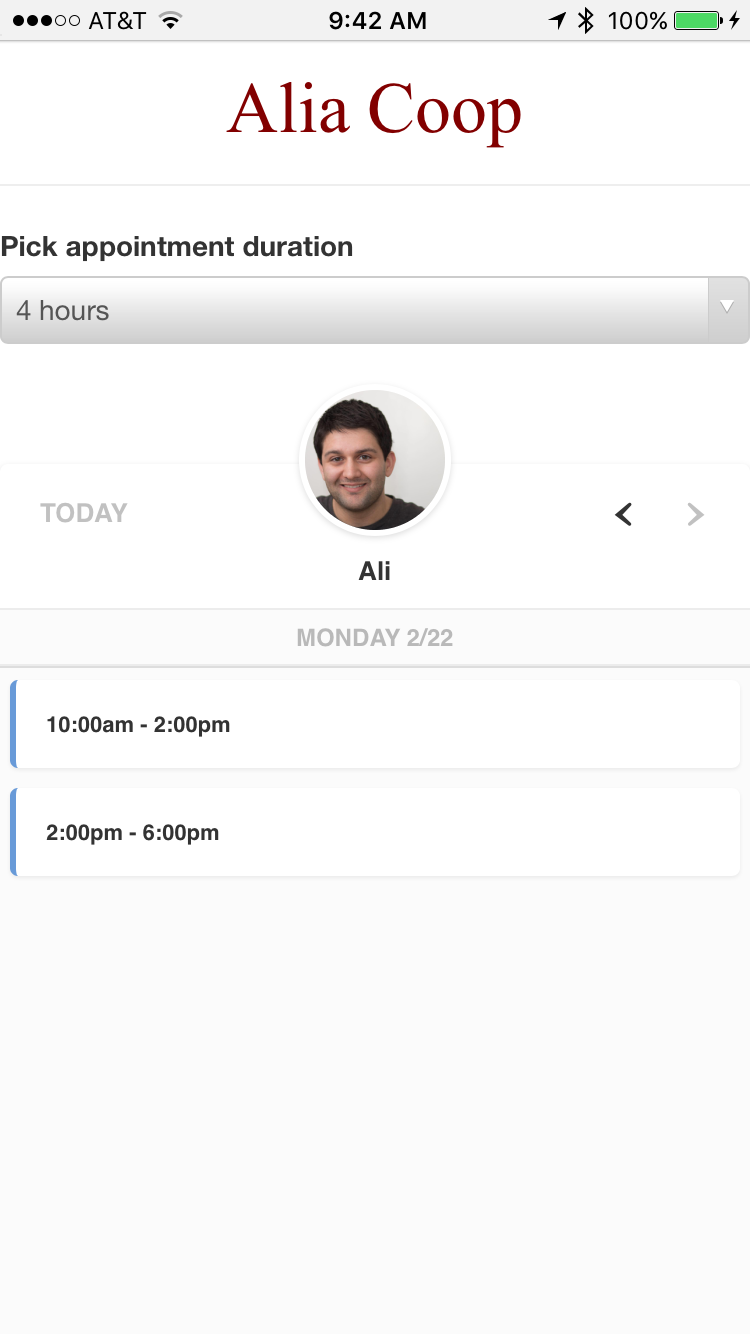
\includegraphics[width=0.24\textwidth]{figures/2.png}
    
\includegraphics[width=0.24\textwidth]{figures/3.png}
\end{SCfigure}
% Figure 1.
% Alia, our prototype cooperative platform for collective governance in a gig marketplace.
% Alia is targeted as a marketplace for domestic workers to do rapid online bookings.
% Its main research goal is to examine affordances for collective decisionmaking and governance in a cooperative marketplace.

The research question that this system asks is: how can distributed, loosely--affiliated workers make effective decisions to govern a cooperative marketplace?
Traditional co--ops operate through scheduled elections to a board and maintain in--group unity via regular or mandatory meetings.
However, worker cooperatives at national and international scales could become unwieldy to govern; empirically, worker cooperatives become proportionally rarer as one looks to larger and larger companies, perhaps in part because the gubernatorial challenges either prevent companies from growing to
(or surviving at)
that scale.

Instead of attempting to scale a single cooperative instance, we propose mechanisms through which local cohorts of workers can `fork' a cooperative's guidelines to create an editable copy, then launch their own co--op.
This new co--op would still operate within the global Alia infrastructure, allowing the proliferation of many local co--ops that benefit from the single central infrastructure.
Examples of projects like this one already exist 
--- Wikipedia's source code, maintained by the Wikimedia Foundation, is available for others to fork and run independently.
Indeed, instantiations of Wikipedia operating under different administrative policies exist: Conservapedia, the Wikia platform, and others illustrate the potential to fork this originating source code and run parallel communities.

We believe that these local groups will be more competent at making decisions rapidly and responsively, while still benefiting from both the network effects of a larger cooperative organization as well as the focus of engineering effort on a single codebase.
If successful, online cooperatives might then be able to scale in ways rarely seen in their offline counterparts.

As Alia begins attracting workers, we will again engage in semi--structured interviews of workers on the platform, surveys and grounded analysis of the platform's forums.
We seek to understand: what issues are most contentious for workers to agree on?

How distributed or centralized do they want the platform's governance to be?
When concerns arise similarly to the externally--owned marketplace, how does the cooperative market deal with them?
We hypothesize that workers will want a loose confederation.
Because workers hold strong self--images as freelancers, they may be wary of systems tightly regulating their behavior.

\section*{Logistics and timeline}
Alia will be open source on GitHub via the MIT license.
The platform will be hosted on Heroku, and data will be secured and privately backed up using Postgres.
The effort will proceed over two years.
In the first year, we will perform the qualitative research with workers in order to understand their platform policy and governance behaviors.
Simultaneously, we will design and implement the first version of the Alia platform.
In the second year, we will launch Alia, grow its use locally in the Bay Area, and perform fieldwork with Alia workers to understand their relationship with the cooperative.
We are thus requesting two years of funding for the pair of graduate students who are leading the project.
They, and the PIs, bring together years of experience in qualitative and historical fieldwork, design and system development.
We are also requesting one month of summer salary funding for each of the PIs to support their work on the project.
If the project is successful in its goals, we may seek a third year of funding to grow the platform nationwide and continue our instrumentation and research on it.

\section*{Policy implications and dissemination strategy}
Our policy and design goal is to understand the kinds of worker collectives that can succeed in an online piecework economy, and to ensure that workers have access to them.
Our research targets will be top--tier venues in human--computer interaction
(e.g., ACM CHI, ACM CSCW)
and political science and sociology
(e.g., APSR, ASR, AJS, AJPS, POP).
One main outlet for broader dissemination will be as part of the Future of Work project at CASBS 
--- which recently published a series of essays in Pacific Standard and placed op eds in important newspapers and online sources; the relevant editors remain keen for new and additional material, and various other magazines
(print and online), such as American Prospect and Boston Review are also interested in possible publication of articles from this project.
A second set of outlets will be through the NDWA's relationships with labor advocates and the press.


\bibliographystyle{apalike}
\bibliography{../references.bib}
\end{document}